\documentclass[11pt,a4paper]{article}

\usepackage[utf8]{inputenc}
\usepackage[T1]{fontenc}
\usepackage{lmodern}
\usepackage[a4paper,margin=2.3cm]{geometry}
\usepackage{amsmath,amssymb}
\usepackage{booktabs}
\usepackage{array}
\usepackage{xcolor}
\usepackage{listings}
\usepackage{enumitem}
\usepackage{fancyhdr}
\usepackage{tikz}
\usetikzlibrary{positioning,arrows.meta,calc}
\usepackage{csquotes}
\MakeOuterQuote{"}
\newcommand{\say}[1]{\enquote{#1}}
\usepackage[hidelinks,colorlinks=true,linkcolor=ColPrim,urlcolor=ColPrim,citecolor=ColPrim]{hyperref}

% ----- Colores -----
\definecolor{ColPrim}{RGB}{30,80,160}
\definecolor{ColSec}{RGB}{200,40,40}
\definecolor{ColGris}{RGB}{90,90,90}
\definecolor{CodeBg}{RGB}{247,247,250}
\definecolor{CodeKw}{RGB}{0,90,160}
\definecolor{CodeStr}{RGB}{160,60,30}
\definecolor{CodeCom}{RGB}{110,120,130}

% ----- Encabezado -----
\pagestyle{fancy}
\fancyhf{}
\lhead{\small\textcolor{ColGris}{Técnicas de ML Supervisado}}
\rhead{\small\textcolor{ColGris}{Máquinas de Soporte Vectorial}}
\cfoot{\thepage}
\renewcommand{\headrulewidth}{0.4pt}

% ----- Estilo de codigo (solo referencial) -----
\lstdefinestyle{py}{
  language=Python,
  backgroundcolor=\color{CodeBg},
  basicstyle=\ttfamily\footnotesize,
  keywordstyle=\color{CodeKw}\bfseries,
  stringstyle=\color{CodeStr},
  commentstyle=\color{CodeCom}\itshape,
  frame=single, rulecolor=\color{gray!40},
  breaklines=true, showstringspaces=false,
  tabsize=4, columns=fullflexible, xleftmargin=10pt,
  framexleftmargin=10pt,
}
\lstset{style=py}

% caja de nota
\newcommand{\nota}[1]{%
  \par\vspace{2pt}\noindent
  \fcolorbox{ColPrim!40}{ColPrim!6}{\parbox{\dimexpr\linewidth-2\fboxsep-2\fboxrule}{\small #1}}\par\vspace{4pt}}

% ----- Portada -----
\title{\vspace{-1.2cm}\textcolor{ColPrim}{\textbf{Máquinas de Soporte Vectorial (SVM)}}\\[4pt]
\large Técnicas de Machine Learning Supervisado}
\author{Michael Lata}
\date{15 de junio de 2026}

\begin{document}
\maketitle
\thispagestyle{fancy}

\noindent\textbf{Resumen.} Este informe se centra en las \textbf{Máquinas de Soporte Vectorial
(SVM)}: su definición e intuición, la formulación matemática del margen máximo, la
regularización mediante el parámetro $C$, el \textbf{truco del kernel} para fronteras no
lineales, su uso en \textbf{clasificación} y \textbf{regresión (SVR)}, y sus aplicaciones.
El código que aparece es \textbf{únicamente de referencia}: muestra cómo se invocaría cada
método, pero no es el objetivo de esta sesión.

\tableofcontents
\vspace{0.3cm}\hrule\vspace{0.4cm}

% ==================================================================
\section{Contexto: clasificación vs.\ regresión}
% ==================================================================
La SVM es una técnica de \textbf{aprendizaje supervisado}: aprende a partir de datos
etiquetados $\{(\mathbf{x}_i, y_i)\}_{i=1}^{N}$. Sirve tanto para:
\begin{itemize}[leftmargin=1.4em,nosep]
  \item \textbf{Clasificación} — la salida es una categoría discreta (ej.\ spam / no spam).
  \item \textbf{Regresión} — la salida es un valor numérico continuo (variante \textbf{SVR}).
\end{itemize}

% ==================================================================
\section{Definición e intuición}
% ==================================================================
Una \textbf{SVM} es un clasificador supervisado que, en lugar de basar la asignación de clase en
distancias a otros puntos, calcula la \textbf{frontera (el hiperplano)} que mejor separa los
grupos. De entre todos los hiperplanos que separan los datos, la SVM elige aquel que
\textbf{maximiza el margen}: la distancia a los puntos más cercanos de cada clase.

\begin{itemize}[leftmargin=1.4em]
  \item Los \textbf{vectores de soporte} son los puntos que definen el margen máximo de
  separación. Son los \textbf{únicos} que determinan el hiperplano; los demás no influyen.
  \item Se llaman \emph{vectores} (y no puntos) porque cada muestra tiene tantos elementos como
  dimensiones tenga el espacio de entrada: es un vector de $n$ dimensiones.
  \item El término \emph{máquina} proviene de \textit{machine learning}.
\end{itemize}

\begin{center}
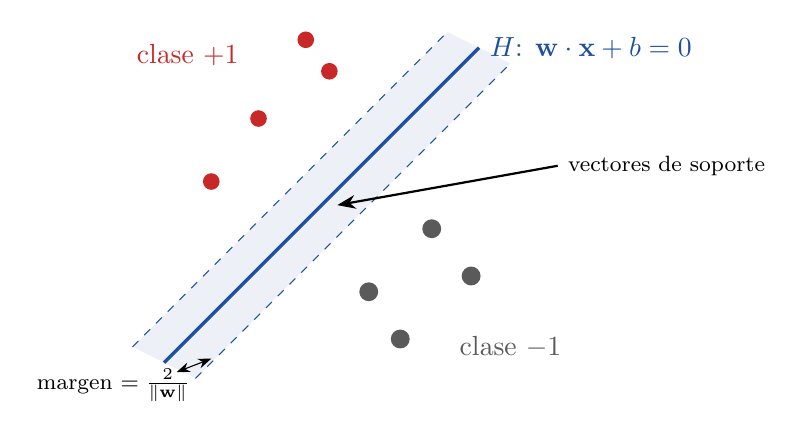
\begin{tikzpicture}[scale=1.0]
  % zona de margen
  \fill[ColPrim!8] (-0.6,-1.7) -- (3.4,2.3) -- (2.6,2.7) -- (-1.4,-1.3) -- cycle;
  \draw[ColPrim,very thick] (-1,-1.5) -- (3,2.5) node[right]{$H$: $\mathbf{w}\cdot\mathbf{x}+b=0$};
  \draw[ColPrim,dashed] (-1.4,-1.3) -- (2.6,2.7);
  \draw[ColPrim,dashed] (-0.6,-1.7) -- (3.4,2.3);
  \foreach \p in {(0.2,1.6),(1.1,2.2),(-0.4,0.8),(0.8,2.6)}
     \fill[ColSec] \p circle (3pt);
  \node[ColSec] at (-0.7,2.4) {clase $+1$};
  \foreach \p in {(1.6,-0.6),(2.4,0.2),(2.0,-1.2),(2.9,-0.4)}
     \draw[fill=white,ColGris,thick] \p circle (3pt);
  \node[ColGris] at (3.4,-1.3) {clase $-1$};
  \draw[->,>=Stealth,thick] (4.0,1.0) node[right]{\footnotesize vectores de soporte} -- (1.2,0.5);
  \draw[<->,>=Stealth] (-0.4,-1.45) -- (-0.84,-1.62) node[midway,below left=-3pt]{\footnotesize margen $=\frac{2}{\|\mathbf{w}\|}$};
\end{tikzpicture}\\[2pt]
{\footnotesize El hiperplano $H$ maximiza la distancia a los puntos más cercanos de ambas clases.
Una muestra nueva se clasifica según el lado de $H$ en el que caiga.}
\end{center}

\nota{\textbf{Idea clave:} los problemas reales tienen muchísimas dimensiones; por eso no se
busca una "línea" sino un \emph{hiperplano} de $n-1$ dimensiones que maximice el margen.}

% ==================================================================
\section{Formulación matemática}
% ==================================================================
El hiperplano se define como $\mathbf{w}\cdot\mathbf{x} + b = 0$, y la regla de decisión es
\[
f(\mathbf{x}) = \operatorname{sign}(\mathbf{w}\cdot\mathbf{x}+b).
\]
La anchura del margen es $2/\|\mathbf{w}\|$, de modo que \textbf{maximizar el margen} equivale a
\textbf{minimizar} $\|\mathbf{w}\|$.

\subsection{Margen duro (datos linealmente separables)}
\begin{equation}
\min_{\mathbf{w},b}\ \tfrac{1}{2}\|\mathbf{w}\|^2
\qquad\text{sujeto a}\qquad y_i(\mathbf{w}\cdot\mathbf{x}_i + b)\ge 1,\ \ \forall i.
\end{equation}

\subsection{Margen blando y regularización (parámetro $C$)}
Es frecuente que los datos tengan ruido, no estén etiquetados perfectamente o sean difíciles de
separar. Para esos casos se permite que algunos puntos violen el margen, introduciendo
\textbf{variables de holgura} $\xi_i \ge 0$:
\begin{equation}
\min_{\mathbf{w},b,\boldsymbol\xi}\ \tfrac{1}{2}\|\mathbf{w}\|^2 + C\sum_{i=1}^{N}\xi_i
\qquad\text{s.a.}\qquad y_i(\mathbf{w}\cdot\mathbf{x}_i + b)\ge 1-\xi_i,\ \ \xi_i\ge 0.
\end{equation}
El hiperparámetro $C$ es la \textbf{penalización del error de entrenamiento} y controla la
regularización:
\begin{center}
\renewcommand{\arraystretch}{1.25}
\begin{tabular}{@{}p{0.46\linewidth}p{0.46\linewidth}@{}}
\toprule
\textcolor{ColPrim}{\textbf{$C$ alto}} & \textcolor{ColSec}{\textbf{$C$ bajo}} \\
\midrule
Penaliza mucho los errores; el modelo se ajusta más al entrenamiento. & Margen más amplio y tolerante a errores. \\
Margen más estrecho. & Mejor generalización en general. \\
Riesgo de \textit{overfitting}. & Riesgo de \textit{underfitting}. \\
\bottomrule
\end{tabular}
\end{center}
En la variante de regresión (SVR) aparece además el parámetro $\varepsilon$ (épsilon), un
\textbf{umbral/threshold}: no se penaliza la predicción mientras el error caiga por debajo de él.

\subsection{Forma dual y vectores de soporte (referencial)}
Resolviendo con multiplicadores de Lagrange $\alpha_i$ se llega al problema \textbf{dual}, que es
donde aparece de forma natural el kernel:
\begin{equation}
\max_{\boldsymbol\alpha}\ \sum_{i}\alpha_i - \tfrac{1}{2}\sum_{i,j}\alpha_i\alpha_j\,y_i y_j\,K(\mathbf{x}_i,\mathbf{x}_j)
\quad\text{s.a.}\quad 0\le\alpha_i\le C,\ \ \sum_i\alpha_i y_i = 0.
\end{equation}
Solo las muestras con $\alpha_i > 0$ son \textbf{vectores de soporte}; el resto no participa en la
predicción. Esto hace la solución compacta y determinista (óptimo global único).

\subsection{Proceso interno: cómo nacen y operan los vectores de soporte}
La pregunta clave es \emph{¿por qué} unos puntos tienen $\alpha_i>0$ y otros $\alpha_i=0$?
La respuesta está en las \textbf{condiciones de Karush--Kuhn--Tucker (KKT)}, que todo óptimo del
problema (2)--(3) debe cumplir. La más importante es la \textbf{holgura complementaria}:
\begin{equation}
\alpha_i\,\bigl[\,y_i(\mathbf{w}\cdot\mathbf{x}_i+b) - 1 + \xi_i\,\bigr]=0,
\qquad
(C-\alpha_i)\,\xi_i = 0.
\end{equation}
De aquí sale \emph{automáticamente} el mecanismo: si un punto está \textbf{estrictamente fuera del
margen} y bien clasificado, el corchete es positivo, así que para cumplir la igualdad
\textbf{obligatoriamente $\alpha_i=0$} y el punto no influye. Solo los puntos que \emph{tocan o
violan} el margen pueden tener $\alpha_i>0$: esos son los vectores de soporte.

\paragraph{Tres tipos de punto.} Las condiciones KKT clasifican cada muestra según su $\alpha_i$:
\begin{center}
\renewcommand{\arraystretch}{1.25}
\begin{tabular}{@{}lll@{}}
\toprule
\textbf{Valor de $\alpha_i$} & \textbf{Posición del punto} & \textbf{Rol} \\
\midrule
$\alpha_i = 0$        & Fuera del margen, bien clasificado & No es vector de soporte (no influye) \\
$0 < \alpha_i < C$    & Justo \emph{sobre} el margen ($\xi_i=0$) & Vector de soporte \textbf{libre} (fija $b$) \\
$\alpha_i = C$        & Dentro del margen o mal clasificado ($\xi_i>0$) & Vector de soporte \textbf{acotado} \\
\bottomrule
\end{tabular}
\end{center}

\paragraph{Reconstrucción de la solución.} El hiperplano se reconstruye \emph{solo} a partir de los
vectores de soporte. De la condición KKT $\mathbf{w}=\sum_i\alpha_i y_i\,\mathbf{x}_i$ y, como los
$\alpha_i=0$ no suman, queda
\begin{equation}
\mathbf{w}=\!\!\sum_{i\in\text{SV}}\!\!\alpha_i y_i\,\mathbf{x}_i,
\qquad
b = y_k - \!\!\sum_{i\in\text{SV}}\!\!\alpha_i y_i\,K(\mathbf{x}_i,\mathbf{x}_k),
\end{equation}
donde $b$ se calcula promediando sobre los vectores de soporte \emph{libres} ($0<\alpha_k<C$), que
son los que caen exactamente sobre el margen. Esto justifica por qué \say{la solución solo depende
de los vectores de soporte}.

\paragraph{Predicción.} Sustituyendo $\mathbf{w}$, la regla de decisión \emph{nunca} usa $\mathbf{w}$
de forma explícita (necesario para el kernel): es una \textbf{suma ponderada solo sobre los vectores
de soporte}:
\begin{equation}
f(\mathbf{x}) = \operatorname{sign}\!\Bigl(\,\sum_{i\in\text{SV}}\alpha_i y_i\,K(\mathbf{x}_i,\mathbf{x}) + b\Bigr).
\end{equation}
Cada vector de soporte \say{vota} con peso $\alpha_i$ según su parecido $K(\mathbf{x}_i,\mathbf{x})$
con la muestra nueva. Por eso menos vectores de soporte $\Rightarrow$ predicción más rápida y, en
general, mejor generalización.

\nota{\textbf{En SVR el proceso es análogo:} los puntos \emph{dentro} del tubo $\varepsilon$ cumplen
la holgura complementaria con $\alpha_i=0$ (no son vectores de soporte); solo los que tocan o salen
del borde del tubo obtienen $\alpha_i>0$ y construyen la función estimada.}

% ==================================================================
\section{El truco del kernel (\textit{kernel trick})}
% ==================================================================
A veces \textbf{no existe} ningún hiperplano que separe las clases en el espacio original: decimos
que las clases \textbf{no son linealmente separables}. El truco del kernel consiste en
\textbf{inventar una dimensión nueva} (proyectar a un espacio de mayor dimensión $\phi(\mathbf{x})$)
en la que las clases sí se puedan separar con un hiperplano. Lo potente es que \textbf{no hace
falta calcular $\phi$ explícitamente}: basta con la función kernel
\[
K(\mathbf{x}_i,\mathbf{x}_j) = \phi(\mathbf{x}_i)\cdot\phi(\mathbf{x}_j).
\]

\begin{center}
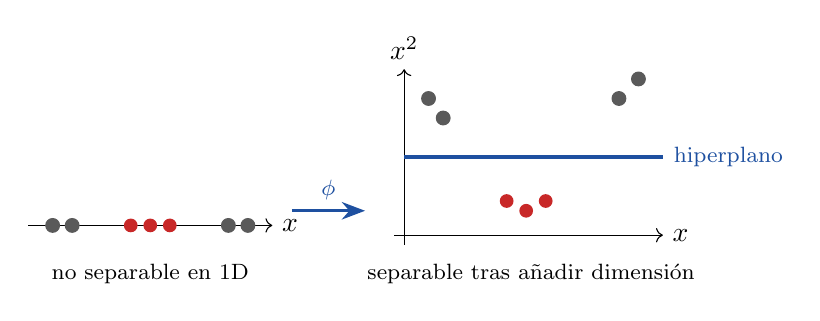
\begin{tikzpicture}[scale=0.62]
  % izquierda: 1D no separable
  \draw[->] (-5.5,0)--(-0.5,0) node[right]{$x$};
  \foreach \x in {-5,-4.6,-1.4,-1.0} \draw[fill=ColGris,ColGris] (\x,0) circle(4pt);
  \foreach \x in {-3.4,-3.0,-2.6} \fill[ColSec] (\x,0) circle(4pt);
  \node at (-3,-1) {\footnotesize no separable en 1D};
  % flecha
  \draw[->,>=Stealth,very thick,ColPrim] (-0.1,0.3)--(1.4,0.3) node[midway,above]{\footnotesize $\phi$};
  % derecha: 2D (x, x^2) separable
  \draw[->] (2,-0.2)--(7.5,-0.2) node[right]{$x$};
  \draw[->] (2.2,-0.4)--(2.2,3.2) node[above]{$x^2$};
  \foreach \x/\y in {2.7/2.6,3.0/2.2,6.6/2.6,7.0/3.0} \draw[fill=ColGris,ColGris] (\x,\y) circle(4pt);
  \foreach \x/\y in {4.3/0.5,4.7/0.3,5.1/0.5} \fill[ColSec] (\x,\y) circle(4pt);
  \draw[ColPrim,very thick] (2.2,1.4)--(7.5,1.4) node[right]{\footnotesize hiperplano};
  \node at (4.8,-1) {\footnotesize separable tras añadir dimensión};
\end{tikzpicture}
\end{center}

\begin{center}
\renewcommand{\arraystretch}{1.45}
\begin{tabular}{@{}lll@{}}
\toprule
\textbf{Kernel} & \textbf{$K(\mathbf{x},\mathbf{x}')$} & \textbf{Uso típico} \\
\midrule
Lineal      & $\mathbf{x}\cdot\mathbf{x}'$ & Datos linealmente separables / muchas \textit{features} \\
Polinómico  & $(\gamma\,\mathbf{x}\cdot\mathbf{x}' + r)^d$ & Fronteras curvas de grado $d$ \\
RBF / Gauss & $\exp(-\gamma\|\mathbf{x}-\mathbf{x}'\|^2)$ & \textbf{Opción por defecto}; fronteras muy flexibles \\
Sigmoide    & $\tanh(\gamma\,\mathbf{x}\cdot\mathbf{x}' + r)$ & Comportamiento similar a una red neuronal \\
\bottomrule
\end{tabular}
\end{center}
\nota{El parámetro $\gamma$ del RBF controla el \emph{alcance} de cada punto: $\gamma$ alto
$\Rightarrow$ fronteras muy locales (riesgo de \textit{overfitting}); $\gamma$ bajo $\Rightarrow$
fronteras más suaves.}

% ==================================================================
\section{SVM para clasificación}
% ==================================================================
\paragraph{Multiclase.} La SVM es binaria por naturaleza. Para más de dos clases se combinan
varios clasificadores: \textbf{one-vs-one} (uno por cada par de clases; el que usa \texttt{libsvm})
o \textbf{one-vs-rest} (uno por clase contra el resto).

\paragraph{Buena práctica.} La SVM es \textbf{muy sensible a la escala} de las variables: siempre
se deben estandarizar las \textit{features} antes de entrenar. Los hiperparámetros se ajustan
normalmente con búsqueda en malla + validación cruzada sobre $C$, $\gamma$ y el kernel.

% ==================================================================
\section{SVM para regresión (SVR)}
% ==================================================================
El mismo concepto se adapta a la regresión: en vez de separar clases, la SVR ajusta una función
dentro de un \textbf{"tubo" de ancho $\varepsilon$} alrededor de los datos. Los puntos que caen
dentro del tubo \textbf{no se penalizan}; solo cuentan los que quedan fuera (que pasan a ser los
vectores de soporte). Se pueden usar los mismos kernels (lineal, polinómico, RBF\dots) para
estimar salidas no lineales.

\begin{center}
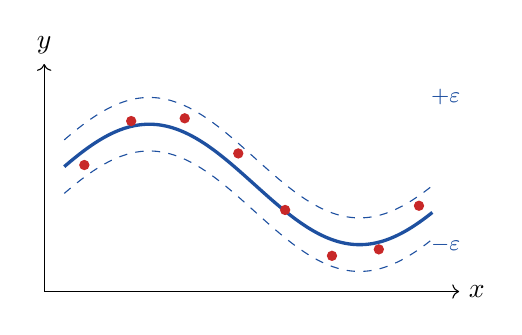
\begin{tikzpicture}[scale=0.85]
  \draw[->] (0,0)--(6.2,0) node[right]{$x$};
  \draw[->] (0,0)--(0,3.4) node[above]{$y$};
  \draw[ColPrim,very thick,domain=0.3:5.8,smooth,samples=60] plot (\x,{1.6+0.9*sin(\x r)});
  \draw[ColPrim,dashed,domain=0.3:5.8,smooth,samples=60] plot (\x,{2.0+0.9*sin(\x r)});
  \draw[ColPrim,dashed,domain=0.3:5.8,smooth,samples=60] plot (\x,{1.2+0.9*sin(\x r)});
  \node[ColPrim] at (6.0,2.9) {\footnotesize $+\varepsilon$};
  \node[ColPrim] at (6.0,0.7) {\footnotesize $-\varepsilon$};
  \foreach \x in {0.6,1.3,2.1,2.9,3.6,4.3,5.0,5.6}
     \fill[ColSec] (\x,{1.6+0.9*sin(\x r)+0.25*sin(7*\x r)}) circle(2.2pt);
\end{tikzpicture}\\[2pt]
{\footnotesize SVR: se penaliza solo lo que sale del tubo de ancho $\varepsilon$.}
\end{center}

% ==================================================================
\section{Aplicaciones y rol histórico}
% ==================================================================
Antes de la era del \textit{deep learning}, las SVM se preferían frente a las redes neuronales
porque sus matemáticas se entienden muy bien y la propiedad del \textbf{margen máximo} resultaba
muy atractiva (las redes estándar de entonces cometían más errores de clasificación). Casos de
éxito clásicos:
\begin{itemize}[leftmargin=1.4em,nosep]
  \item Reconocimiento óptico de caracteres (OCR).
  \item Detección de rostros para el enfoque automático de cámaras digitales.
  \item Filtros de spam de correo electrónico.
  \item Clasificación de imágenes satelitales (nubes, tierra, agua, hielo\dots).
\end{itemize}
Actualmente las \textbf{redes neuronales profundas} suelen superar a las SVM en capacidad de
aprendizaje y generalización, pero la SVM sigue siendo muy útil con \textbf{pocos datos} o
\textbf{muchas dimensiones}.

% ==================================================================
\section{Ventajas y desventajas}
% ==================================================================
\begin{center}
\renewcommand{\arraystretch}{1.3}
\begin{tabular}{@{}p{0.47\linewidth}p{0.47\linewidth}@{}}
\toprule
\textcolor{ColPrim}{\textbf{Ventajas}} & \textcolor{ColSec}{\textbf{Desventajas}} \\
\midrule
Muy eficaz en espacios de alta dimensión. & Costosa en datasets muy grandes ($\sim O(N^2)$–$O(N^3)$). \\
Robusta al \textit{overfitting} con un $C$ bien ajustado. & Sensible a la elección del kernel y de $C$, $\gamma$. \\
Solución determinista (óptimo global único). & Requiere estandarizar las variables. \\
Compacta: solo depende de los vectores de soporte. & Poco interpretable; no da probabilidades de forma directa. \\
Maneja no linealidad con el kernel trick. & Ajuste de hiperparámetros laborioso. \\
\bottomrule
\end{tabular}
\end{center}

% ==================================================================
\section{Código de referencia}
% ==================================================================
\nota{\textbf{Nota:} esta sección es \emph{solo de referencia}. Muestra cómo se invocaría la SVM
en \texttt{scikit-learn}; no es necesario ejecutar nada en esta sesión.}

\subsection*{Clasificación (referencial)}
\begin{lstlisting}
from sklearn.svm import SVC
from sklearn.preprocessing import StandardScaler
from sklearn.pipeline import make_pipeline

# Escalado obligatorio + SVM con kernel RBF
clf = make_pipeline(
    StandardScaler(),
    SVC(kernel='rbf', C=1.0, gamma='scale')  # C: regularizacion; gamma: alcance RBF
)
clf.fit(X_train, y_train)
y_pred = clf.predict(X_test)
\end{lstlisting}

\subsection*{Regresión SVR (referencial)}
\begin{lstlisting}
from sklearn.svm import SVR

svr = SVR(kernel='rbf', C=100, gamma=0.1, epsilon=0.1)  # epsilon = ancho del tubo
svr.fit(X_train, y_train)
\end{lstlisting}

% ==================================================================
\section*{Referencias}
\addcontentsline{toc}{section}{Referencias}
\small
\begin{enumerate}[leftmargin=1.6em,label={[\arabic*]}]
  \item C.\ Cortes, V.\ Vapnik. \textit{Support-Vector Networks}. Machine Learning, 1995.
  \item B.\ Schölkopf, A.\ J.\ Smola. \textit{Learning with Kernels: Support Vector Machines,
  Regularization, Optimization, and Beyond}. MIT Press, 2001.
  \item C.\ Bishop. \textit{Pattern Recognition and Machine Learning}. Springer, 2006.
  \item S.\ Raschka, V.\ Mirjalili. \textit{Python Machine Learning}. Packt Publishing, 2017.
\end{enumerate}

\end{document}
